\documentclass{article}
\usepackage{KJN}
\usepackage{a4wide,changebar}
\usepackage[numbered,framed]{mcode}

\title{BRISK-based Natural Landmark Localisation for Robocup}
\author{Daniel Mankowitz: S1128165}
\date{3/11/2011}

\begin{document}
\maketitle

\newpage
\begin{abstract}
This is the abstract
\end{abstract}

\section{Introduction}
\label{sec:introduction}

\subsection{Background}
\label{sec:background}

\section{General Feature Extraction Techniques}
\label{sec:genFeatureExtract}

\subsection{2DSURF}
\label{sec:2dsurf}

\subsubsection{Detector}
\label{2dsurfdetect}

\subsubsection{Descriptor}
\label{2dsurfdescribe}

\subsection{BRISK}
\label{sec:brisk}

\subsubsection{Detector}
\label{briskDetect}

\subsubsection{Descriptor}
\label{briskDescribe}

\subsection{BRISK-2DSURF}
\label{sec:brisk2dsurf}

\subsubsection{Detector}
\label{brisk2dsurfDetect}

\subsubsection{Descriptor}
\label{brisk2dsurfDescribe}


\section{Feature Matching}
\label{sec:matching}

\subsection{K-Nearest Neighbours}
\label{sec:knn}

\subsection{Hamming Distance}
\label{sec:hamming}

\subsection{Euclidean Distance}
\label{sec:euclidean}

\subsection{Matching Validation}
\label{sec:validation}

\subsubsection{K-Nearest Neighbors Criterion}
\label{sec:knnMatching}

\subsubsection{Angle and Distance Constraints}
\label{sec:angleDistanceConstraints}

\section{Robocup Feature Extraction Techniques}
\label{sec:realtimeFeatureExtraction}

\subsection{S-BRISK}
\label{sec:sbrisk}

\subsubsection{Detector}
\label{sbriskDetect}

\subsubsection{Descriptor}
\label{sbriskDescribe}

\subsubsection{Matching}
\label{sbriskMatching}

\subsection{1DSURF}
\label{sec:1dsurf}

\subsubsection{Detector}
\label{1dsurfDetect}

\subsubsection{Descriptor}
\label{1dsurfDescribe}

\subsubsection{Matching}
\label{1dsurfMatching}

\section{Localisation Algorithm}
\label{sec:localisation}

\section{Experiments and Results}
\label{sec:experimentsResults}

\subsection{Feature Extraction Performance}
\label{sec:featureExtraction}
The setup for the feature extraction experiments is as follows. Four image datasets were generated. These images were taken from the Nao's camera at different angles and scales in order to ensure realistic images similar to those taken in a robocup soccer game. The first dataset is of the area to the left of the player's goal. The second dataset is to the right of the player's goal. The third and fourth datasets are to the left and right of the opponents goal respectively.\\

Feature detection, extraction and matching routines were performed on pairs of images to determine whether the images match or not. Pairs of images taken from the same dataset are referred to as overlapping images. An image is considered to overlap another image if at least four major landmarks are identified in both images. Pairs of images taken from different datasets are referred to as non-overlapping images. In order to ensure that images do not overlap, datasets from opposite sides of the soccer field were compared. Thus dataset one and two were compared with datasets three and four respectively as shown in \tabref{table:overlap}. \\

In total, $108$ overlapping images were used to generate $1421$ overlapping image pairs. A further $108$ non-overlapping images were used to generate $1209$ non-overlapping image pairs.\\ 

The overlapping image pairs are initially used to determine the optimal parameters for the feature extraction algorithms. Once the optimal parameters have been found, both the non-overlapping image pairs and the overlapping image pairs are used to determine the matching performance of the respective feature extraction algorithm.\\

\begin{table}
\caption{Datasets and image combinations used for the comparison tests}
\begin{tabular}{|c|c|c|c|c|}
\hline 
Dataset A & Dataset B & Images in A & Images in B & Compared Image Pairs\tabularnewline
\hline 
\hline 
\multicolumn{5}{|c}{Overlapping Images}\tabularnewline
\hline 
1 & 1 & 26 & 26 & 325\tabularnewline
\hline 
2 & 2 & 28 & 28 & 378\tabularnewline
\hline 
3 & 3 & 31 & 31 & 465\tabularnewline
\hline 
4 & 4 & 23 & 23 & 253\tabularnewline
\hline 
\multicolumn{2}{|c|}{Total} & 108 & 108 & 1421\tabularnewline
\hline 
\multicolumn{5}{|c}{Non-Overlapping Images}\tabularnewline
\hline 
1 & 3 & 26 & 31 & 325\tabularnewline
\hline 
1 & 4 & 26 & 23 & 253\tabularnewline
\hline 
2 & 3 & 28 & 31 & 378\tabularnewline
\hline 
2 & 4 & 28 & 23 & 253\tabularnewline
\hline 
\multicolumn{2}{|c|}{Total} & 108 & 108 & 1209\tabularnewline
\hline 
\end{tabular}
\label{table:overlap}
\end{table}

\subsubsection{Finding the Optimal Detection Parameters}
\label{sec:optimalParameters}
%Describes how to find the optimal hamming distance, euclidean distance, and response thresholds for each method
Before the feature extraction and matching algorithm can be performed, the optimal set of detection parameters for the algorithm need to be determined. The detection parameters can be thresholds, hamming distances or euclidean distances as discussed in \secref{sec:matching}. Four datasets containing in total $108$ overlapping images were used to determine the optimum feature extraction parameters. All possible combinations of overlapping images were matched in datasets one to four for various detection parameter values. A procedure has been developed in order to calculate the optimum detection parameters used to provide the best matching performance.\\
%The equation containing the optimal parameters
In order to find the optimal detection parameters, the Single Image Score (SIS) needs to be computed. This equation is shown in \eqnref{eqn:optimalParameters}. This matching score represents how good at match is between the $i^{th}$ pair of images in a particular dataset for a certain set of detection parameters. For example, if the detector used is BRISK, then the $SIS_{i}$ presents the matching score for the $i^{th}$ pair of images for a specific detection threshold as mentioned in \secref{sec:brisk}. \\

\begin{equation}
SIS_{i} = \frac{k_1 f(t_{i}) + k_2 g_(NVM_{i})}{k_1 + k_2}
\label{eqn:optimalParameters}
\end{equation}

This matching score is composed of two normalised scoring functions, namely $f(t_{i})$ and $g(NVM_{i})$ shown in \eqnref{eqn:time} and \eqnref{eqn:nvm} respectively. $f(t_{i})$ represents the matching score for the $i^{th}$ pair of images for a particular dataset based on the time, $t$, taken to perform the detection, extraction and matching routines respectievly between these images. The unit of $t$ is milliseconds and the value of $t$ is normalised to a scale between $0$ and $0.83$ by dividing it by $1.2 t_{max}$ where $t_{max}$ is the largest time tabulated for the current dataset in milliseconds. A value of $0.1$ has been added to this ratio in order to prevent $log(0) = \infty$ which would largely bias the results. The factor of $1.2$ has been added in order to ensure that the term $\frac{t}{1.2 t_{max}} + 0.1$ stays below a value of $1$. This will ensure that, for large $t$, meaning that the algorithm takes a large amount of time to perform the routine, the matching score will be low, whereas for small $t$, the matching score will be high. \\

The second scoring function used to calculate the SIS is $g(NVM_{i})$. This scoring function rewards the $i^{th}$ pair of images if they contain a large amount of valid matches. This is intuitive as the more valid matches there are between two images, the more certain the match becomes. The variable $NVM$ represents the Number of Valid Matches (NVM) between two images. This function is normalised between $0$ and  $0.9$ by the total amount of matches, $M_{total}$, that are generated for the $i^{th}$ image pair. The reason $M_{total}$ has been chosen as the normalisation factor is because it prevents a biased score. A biased score can occur if a pair of images generate a large amount of matches, but only a small percentage of the matches are valid. However, the resulting number of valid matches may be larger than another pair of images that generated a small set of matches, but a high proportion of valid matches. Thus calculating the above-mentioned relative ratio will prevent image pairs with a large number of matches from dominating image pairs with a smaller number of matches. The value $0.1$ has been added to ensure that no infinite scores are computed.\\ 

The parameters $k_1$ and $k_2$ are weights that are used to bias the effects of the two scoring functions. Thus they can be used as controls to determine whether time or valid matches should have a larger influence on the matching score. The weights sum to one and are used to normalise the SIS function.\\

\begin{equation}
f(t_{i}) = \mid log_{10}(\frac{t}{1.2 t_{max}} + 0.1) \mid \quad f(t_{i})\epsilon [0, 1]
\label{eqn:time}
\end{equation}

\begin{equation}
g(NVM_{i}) = \frac{NVM}{M_{total} + 0.1} \quad g(NVM_{i}) \epsilon [0, 0.9]
\label{eqn:nvm}
\end{equation}

Once the SIS score has been calculated for each pair of images in a particular dataset, the scores are then summed together for specific sets of detection parameter values. The resulting score is called the Multi-Image Score (MIS) and is shown in \eqnref{eqn:mims}.\\

\begin{equation}
MIS = \frac{k_3 \frac{\sum_{i=1}^{n} SIMS_{i}}{N} + k_4 h(NZM)}{k_3 + k_4}
\label{eqn:mims}
\end{equation}

The MIS score includes the computation of the mean of all SIMS scores for a particular set of detection parameter values. A function has been introduced to account for the Number of Zero Matches (NZM) for a particular set of detection parameter values. An NZM is defined as a pair of images containing no valid matches. The function $h(NZM)$ is defined in \eqnref{eqn:nzm}. This equation has the same form as equation \eqnref{eqn:time} and therefore behaves in the same way. Detection parameters containing a large number of NZMs are penalised by this function since NZMs should not be present in a dataset of overlapping images. \\

\begin{equation}
h(NZM) = \mid log_{10}(\frac{NZM}{1.2 NZM_{max}} + 0.1) \mid \quad h(NZM)\epsilon [0, 1]
\label{eqn:nzm}
\end{equation}

The MIS score contains another set of weighting parameters, $k_3$ and $k_4$, that can again be used to control the influence of each term in the function. These weights add up to one.\\

\eqnref{eqn:mims} therefore provides an overall score of how well images are matched for a specific setting of detection parameter values. The feature detection parameters corresponding to the maximum MIS score are selected as the optimal detection parameters to be used in the feature extraction procedure.\\

%Could possibly add in the addition of averaging the mScore matrices and then finding the maximum value. The advantage of this is to find the most consistent radius and threshold.  

%The optimal parameter graphs
\begin{figure}[h!]
\begin{minipage}[b]{0.5\linewidth}
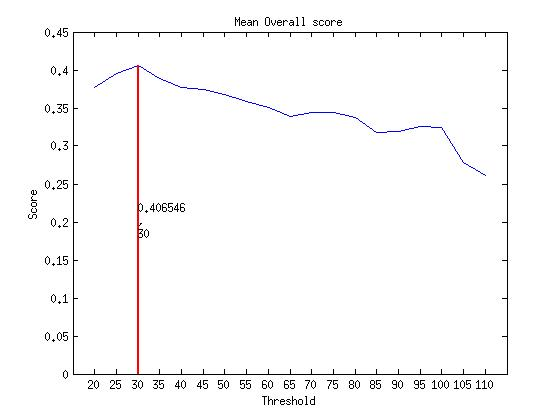
\includegraphics[scale=0.5]{../Drawings/OptimalParameters_SBRISK_SBRISK_KNN.jpg}
\caption{The optimal parameters for S-BRISK with KNN}
\label{fig:sbriskknnOptimal}
\end{minipage}
\hspace{0.5cm}
\begin{minipage}[b]{0.5\linewidth}
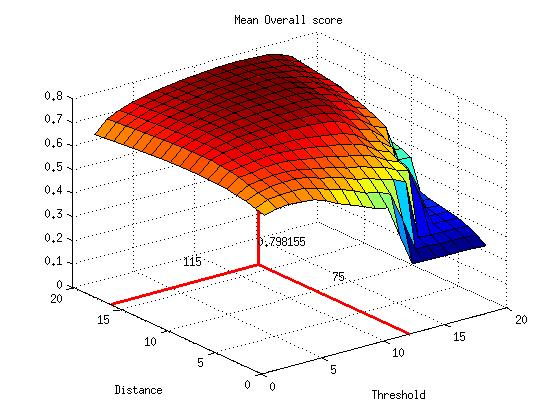
\includegraphics[scale=0.5]{../Drawings/OptimalParameters_SBRISK_SBRISK_hamming.jpg}
\caption{The optimal parameters for S-BRISK with Hamming Distance}
\label{fig:sbriskHammingOptimal}
\end{minipage}
\begin{minipage}[b]{0.5\linewidth}
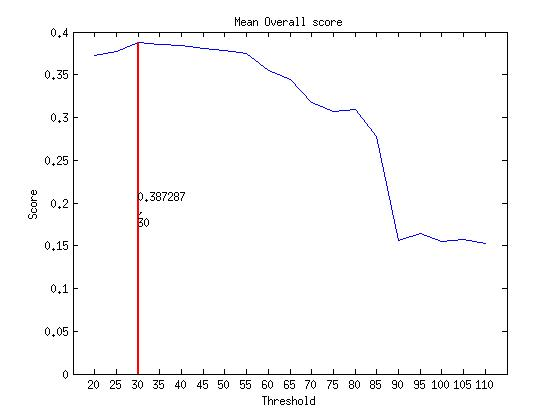
\includegraphics[scale=0.5]{../Drawings/OptimalParameters_BRISK4_BRISK4_KNN.jpg}
\caption{The optimal parameters for BRISK4 with KNN Distance}
\label{fig:sbriskHammingOptimal}
\end{minipage}
\begin{minipage}[b]{0.5\linewidth}
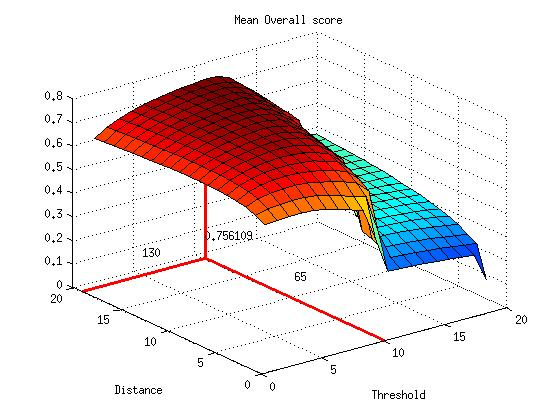
\includegraphics[scale=0.5]{../Drawings/OptimalParameters_BRISK4_BRISK4_Hamming.jpg}
\caption{The optimal parameters for BRISK4 with Hamming Distance}
\label{fig:sbriskHammingOptimal}
\end{minipage}
\begin{minipage}[b]{0.5\linewidth}
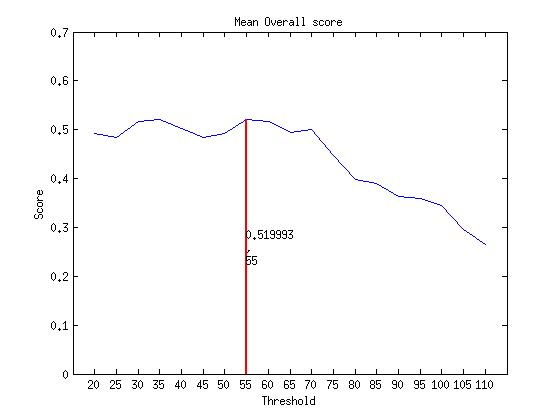
\includegraphics[scale=0.5]{../Drawings/OptimalParameters_SBRISK_SURF2D_KNN.jpg}
\caption{The optimal parameters for SBRISK SURF2D with KNN}
\label{fig:sbriskHammingOptimal}
\end{minipage}
\end{figure}

\begin{table}
\caption{The optimal thresholds for the 2-KNN feature extraction algorithms}
\begin{tabular}{|c|c|c|c|c|c|c|c|c|}
\hline 
Detector & Extractor & Matcher & k1 & k2 & k3 & k4 & Normal threshold & Consistent threshold\tabularnewline
\hline 
\hline 
S-BRISK & S-BRISK & KNN=2 & 0.6 & 0.4 & 0.4 & 0.6 & 46.25 & 30\tabularnewline
\hline 
BRISK4 & BRISK4 & KNN=2 & 0.6 & 0.4 & 0.4 & 0.6 & 51.25 & 30\tabularnewline
\hline 
SBRISK & SURF2D & KNN=2 & 0.6 & 0.4 & 0.4 & 0.6 & 45 & 35\tabularnewline
\hline 
\end{tabular}
\label{tab:knnStatistics}
\end{table}

\begin{table}
\caption{The optimal thresholds for the Hamming/Euclidean distance feature extraction algorithms}
\begin{tabular}{|c|c|c|c|c|c|c|c|c|c|c|}
\hline 
Detector & Extractor & Matcher & k1 & k2 & k3 & k4 & threshold & distance & thresholdC & distanceC\tabularnewline
\hline 
\hline 
S-BRISK & S-BRISK & Hamming & 0.6 & 0.4 & 0.4 & 0.6 & 78.75 & 110 & 75 & 115\tabularnewline
\hline 
BRISK4 & BRISK4 & Hamming & 0.6 & 0.4 & 0.4 & 0.6 & 85 & 121.25 & 130 & 65\tabularnewline
\hline 
SBRISK & SURF2D & Euclidean & 0.6 & 0.4 & 0.4 & 0.6 & 65 & 0.28 & 60 & 0.28\tabularnewline
\hline 
\end{tabular}
\label{tab:hammingStatistics}
\end{table}

\subsubsection{Matching Score}
\label{sec:matchingScore}
As mentioned in \secref{sec:matching}, in the case of 2D SURF, keypoint pairs can be matched based on the euclidean distance between the feature vectors representing the keypoints. Similarly, in the case of BRISK, keypoints can be matched based on the hamming distance between the feature vectors. In both cases, taking the inverse distance can produce a matching score as shown in \eqnref{eqn:inverseDistance}. The smaller the distance between feature vectors, the more similar the keypoints become resulting in a high matching score and vice versa. In order to determine whether or not this score is a good metric for classifying whether images match or not, a number of tests were performed.

\begin{equation}
Score = \frac{1}{distance}
\label{eqn:inverseDistance}
\end{equation}

Utilising the images from the datasets in \tabref{table:overlap}, matching scores were computed for pairs of overlapping images and pairs of non-overlapping images respectively. It was expected that the matching score for the overlapping images would be larger than that of the non-overlapping images. \\

Various feature extraction methods were performed on all possible combinations of overlapping and non-overlapping image pairs respectively. These include SBRISK, BRISK4 and SBRISK-SURF2D. The matching criteria utilised was either K-Nearest Neighbors (KNN), Euclidean distance or Hamming distance depending on the method. The mean matching scores for $1421$ overlapping images and $1209$ non-overlapping images are shown in \tabref{tab:matchingScoreCompare}.

\begin{table}
\begin{tabular}{|c|c|c|c|}
\hline 
Method & Matching Technique & Overlapping Score & Non-overlapping Score\tabularnewline
\hline 
\hline 
SBRISK & KNN & 0.3257 & 0.0048\tabularnewline
\hline 
 & Hamming Distance & 0.1201 & 0.0051\tabularnewline
\hline 
BRISK4 & KNN & 0.1666 & 0.0024\tabularnewline
\hline 
 & Hamming Distance & 0.1652 & 0.0071\tabularnewline
\hline 
SBRISK- SURF2D & KNN & 64.34 & 3.40\tabularnewline
\hline 
 & Euclidean Distance & 55.02 & 1.38\tabularnewline
\hline 
\end{tabular}
\label{tab:matchingScoreCompare}
\end{table}

\subsubsection{Keypoint Matching Properties}
\label{sec:keypointMatching}
%The mean distance between 
In order to determine whether or not matches in images are valid, two techniques have been implemented as discussed in \secref{sec:validation}. The first technique is the angle and distance constraint and the second is the KNN ratio. Utilising these techniques, overlapping image pairs were tested using SBRISK with a threshold of $46.25$ (which is the optimal threshold according to the method in \secref{sec:optimalParameters}).\\

The keypoints corresponding to valid and invalid matches in each of the images respectively were recorded. This was performed in order to determine whether or not keypoints corresponding to a valid match have different properties compared to keypoints corresponding to an invalid match. Three criteria were analysed, namely the angle, size and response of each matched keypoint. The mean angle, size and response as well as the standard deviation for each of these keypoints were calculated over $56$ image pairs from all four datasets. In total, $748$, valid keypoint matches were utilised and $3847$ invalid keypoint matches were used in the calculations.\\

%The keypoints in image A were subtracted from the keypoints in image B.

It was found that the valid matched keypoints

%A picture of the graph for each method containing the optimal parameters

\begin{table}
\begin{tabular}{|c|c|c|c|c|}
\hline 
Method & Total Matches & Valid Matches & Invalid Matches & Best matches\tabularnewline
\hline 
\hline 
SBRISK - 2KNN & 106.96 & 5.34 & 101.62 & 3.24\tabularnewline
\hline 
BRISK4 - 2KNN & 105.44 & 4.63 & 100.81 & 2.65\tabularnewline
\hline 
SBRISK-SURF2D - 2KNN & 132.62 & 7.13 & 125.48 & 4.72\tabularnewline
\hline 
\end{tabular}
\label{tab:keypointsMatchesKNN}
\end{table}

\begin{table}
\begin{tabular}{|c|c|c|c|c|}
\hline 
Method & Total Matches & Valid Matches & Invalid Matches & Best matches\tabularnewline
\hline 
\hline 
SBRISK - Hamming & 32.20 & 17.05 & 15.14 & 6.10\tabularnewline
\hline 
BRISK4 - Hamming & 30.68 & 18.70 & 11.98 & 5.21\tabularnewline
\hline 
SBRISK-SURF2D - Euclidean & 11.61 & 7.16 & 4.44 & 4.93\tabularnewline
\hline 
\end{tabular}
\label{tab:keypointsMatchesHamming}
\end{table}

\subsubsection{Overall Classification Performance}
\label{sec:rocCurves}

\begin{figure}[h!]
\begin{minipage}[b]{0.5\linewidth}
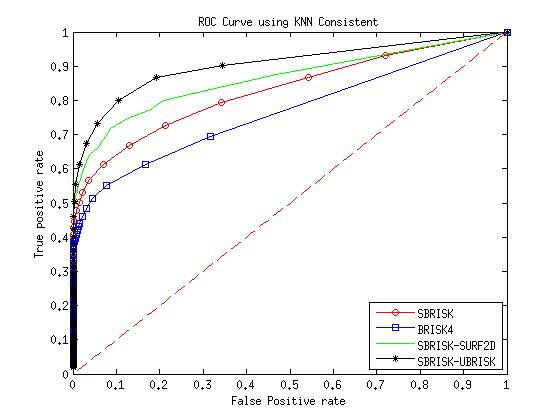
\includegraphics[scale=0.5]{../Drawings/ROC_General_Hamming.jpg}
\caption{A comparison of the ROC curves for SBRISK, BRISK4 and SBRISK-SURF2D using Hamming distance for matching}
\label{fig:compareHamming}
\end{minipage}
\hspace{0.5cm}
\begin{minipage}[b]{0.5\linewidth}
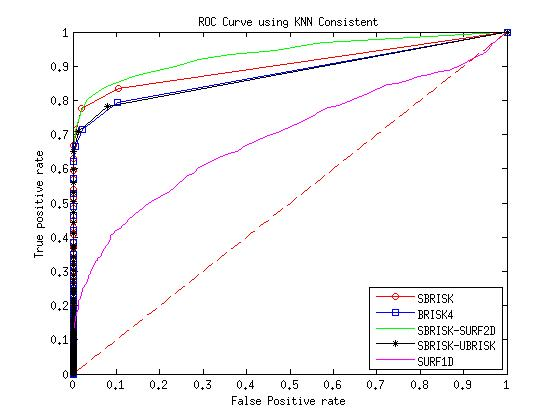
\includegraphics[scale=0.5]{../Drawings/ROC_General_KNN.jpg}
\caption{A comparison of the ROC curves for SBRISK, BRISK4 and SBRISK-SURF2D using 2-KNN for matching}
\label{fig:compareKNN}
\end{minipage}
\begin{minipage}[b]{0.5\linewidth}
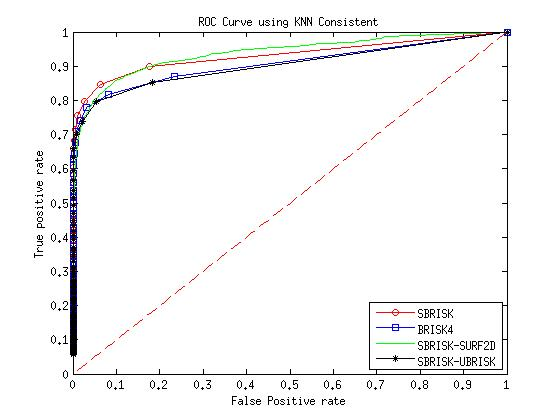
\includegraphics[scale=0.5]{../Drawings/ROC_General_KNN_Consistent.jpg}
\caption{A comparison of the ROC curves for SBRISK, BRISK4 and SBRISK-SURF2D using 2-KNN for matching and consistent thresholds}
\label{fig:compareKNNConsistent}
\end{minipage}
\end{figure}

\begin{table}
\caption{The performance statistics of 2-KNN feature extraction algorithms}
\begin{tabular}{|c|c|c|c|c|c|c|c|c|c|c|}
\hline 
Method (2-KNN) & Threshold & \% AUC & Detection(ms) & Extraction(ms) & Matching(ms) & Verification(ms) & Overall(ms) & OP & \% TP & \% FP\tabularnewline
\hline 
\hline 
SBRISK & Normal & 90.31 & 5.85 & 8.79 & 1.89 & 0.04 & 24.98 &  &  & \tabularnewline
\hline 
 & Consistent & 93.06 & 7.07 & 17.08 & 6.52 & 0.05 & 39.17 &  &  & \tabularnewline
\hline 
BRISK4 & Normal & 88.08 & 19.43 & 9.34 & 1.54 & 0.03 & 39.06 &  &  & \tabularnewline
\hline 
 & Consistent & 90.76 & 27.79 & 18.00 & 6.81 & 0.05 & 61.30 &  &  & \tabularnewline
\hline 
SBRISK - SURF2D & Normal & 93.53 & 6.07 & 17.99 & 0.54 & 0.03 & 33.26 &  &  & \tabularnewline
\hline 
 & Consistent & 93.79 & 7.00 & 32.86 & 1.45 & 0.06 & 49.78 &  &  & \tabularnewline
\hline 
\end{tabular}
\label{tab:keypointsMatchesHamming}
\end{table}

\begin{table}
\caption{The performance statistics of Hamming/Euclidean Distance feature extraction algorithms}
\begin{tabular}{|c|c|c|c|c|c|c|c|c|c|c|}
\hline 
Method & Threshold, distance & \% AUC & Detection(ms) & Extraction(ms) & Matching(ms) & Verification(ms) & Overall(ms) & OP & \% TP & \% FP\tabularnewline
\hline 
\hline 
SBRISK & Normal & 82.24 & 5.15 & 4.62 & 0.33 & 0.01 & 18.63 &  &  & \tabularnewline
\hline 
BRISK4 & Normal & 74.36 & 14.55 & 4.42 & 0.26 & 0.01 & 27.87 &  &  & \tabularnewline
\hline 
SBRISK-SURF2D & Normal & 87.37 & 16.7 & 87.19 & 0.43 & 0.01 & 112.97 &  &  & \tabularnewline
\hline 
\end{tabular}
\label{tab:hammingStatistics}
\end{table}





\subsubsection{SURF2D}
\label{sec:2dsurfResults}
%1. Picture of the ROC curve
%STATS:
%a. The AUC
%b. average time, extraction, deletion
%c. Performance under lighting, scale, rotation and image blur

\subsubsection{BRISK}
\label{sec:briskResults}
%Find the optimal parameters:
%1. threshold only + KNN
%\begin{table}
%\caption{Optimum Threshold}
%\begin{tabular}{|c|c|c|c|c|c|c|c|c|}
%\hline 
%Detector & Extractor & Matcher & k1 & k2 & k3 & k4 & threshold & thresholdC\tabularnewline
%\hline 
%\hline 
%BRISK4 & BRISK4 & KNN=2 & 0.6 & 0.4 & 0.4 & 0.6 & 51.25 & 30\tabularnewline
%\hline 
%\end{tabular}
%\label{tab:sbrisk}
%\end{table}

%\begin{figure}[h!]
%	\centering
%		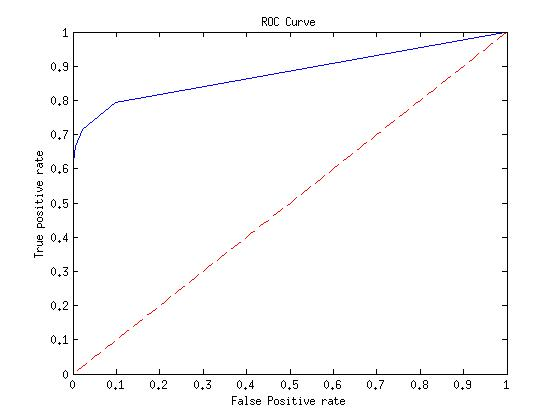
\includegraphics[width=0.6\textwidth]{../Drawings/ROC_BRISK4_BRISK4_KNN.jpg}
%	\caption{The ROC Curve for BRISK4 KNN}
%	\label{fig:sbriskroc}
%\end{figure}

%\begin{table}
%\caption{Optimum Threshold}
%\begin{tabular}{|c|c|c|c|c|c|c|c|c|}
%\hline 
%\% AUC & Detection(ms) & Extraction(ms) & Matching(ms) & Verification(ms) & Overall(ms) & OP & \% TP & \% FP\tabularnewline
%\hline 
%\hline 
%88.08 & 19.43 & 9.34 & 1.54 & 0.03 & 39.06 &  &  & \tabularnewline
%\hline 
%90.76 & 27.79 & 18.00 & 6.81 & 0.05 & 61.30 &  &  & \tabularnewline
%\hline 
%\end{tabular}
%\label{tab:sbrisk}
%\end{table}

%2. threshold, hammingdistance + KNN
%****************************************************************
%\begin{table}
%\caption{Optimum Threshold}
%\begin{tabular}{|c|c|c|c|c|c|c|c|c|c|c|}
%\hline 
%Detector & Extractor & Matcher & k1 & k2 & k3 & k4 & threshold & distance & thresholdC & distanceC\tabularnewline
%\hline 
%\hline 
%BRISK4 & BRISK4 & Hamming & 0.6 & 0.4 & 0.4 & 0.6 & 85 & 121.25 & 130 & 65\tabularnewline
%\hline 
%\end{tabular}
%\label{tab:sbrisk}
%\end{table}

%1. Picture of the ROC curve
%STATS:
%a. The AUC
%b. average time, extraction, deletion
%\begin{figure}[h!]
%	\centering
%		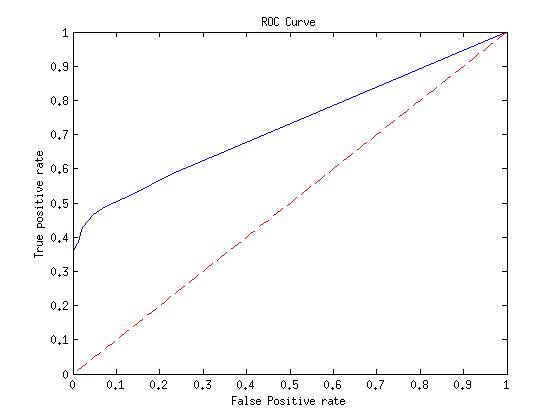
\includegraphics[width=0.6\textwidth]{../Drawings/ROC_BRISK4_BRISK4_Hamming.jpg}
%	\caption{The ROC Curve for BRISK4 Hamming}
%	\label{fig:sbriskroc}
%\end{figure}

%\begin{table}
%\caption{Optimum Threshold}
%\begin{tabular}{|c|c|c|c|c|c|c|c|c|}
%\hline 
%\% AUC & Detection(ms) & Extraction(ms) & Matching(ms) & Verification(ms) & Overall(ms) & OP & \% TP & \% FP\tabularnewline
%\hline 
%\hline 
%74.36 & 14.55 & 4.42 & 0.26 & 0.01 & 27.87 &  &  & \tabularnewline
%\hline 
%\end{tabular}
%\end{table}


\subsubsection{BRISK-SURF2D}
\label{sec:brisk2dsurfResults}
%1. Picture of the ROC curve

%\begin{table}
%\caption{Optimum Threshold}
%\begin{tabular}{|c|c|c|c|c|c|c|c|c|}
%\hline 
%Detector & Extractor & Matcher & k1 & k2 & k3 & k4 & threshold & thresholdC\tabularnewline
%\hline 
%\hline 
%SBRISK & SURF2D & KNN=2 & 0.6 & 0.4 & 0.4 & 0.6 & 45 & 35\tabularnewline
%\hline 
%\end{tabular}
%\label{tab:sbrisk}
%\end{table}

%\begin{figure}[h!]
%	\centering
%		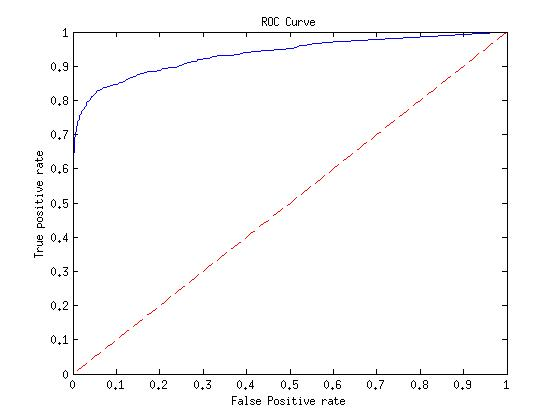
\includegraphics[width=0.6\textwidth]{../Drawings/ROC_SBRISK_SURF2D_KNN.jpg}
%	\caption{The ROC Curve for SBRISK SURF2D KNN}
%	\label{fig:sbriskroc}
%\end{figure}


%\begin{table}
%\caption{Optimum Threshold}
%\begin{tabular}{|c|c|c|c|c|c|c|c|c|}
%\hline 
%\% AUC & Detection(ms) & Extraction(ms) & Matching(ms) & Verification(ms) & Overall(ms) & OP & \% TP & \% FP\tabularnewline
%\hline 
%\hline 
%93.53 & 6.07 & 17.99 & 0.54 & 0.03 & 33.26 &  &  & \tabularnewline
%\hline 
%93.79 & 7.00 & 32.86 & 1.45 & 0.06 & 49.78 &  &  & \tabularnewline
%\hline 
%\end{tabular}
%\end{table}
%STATS:
%a. The AUC
%b. average time, extraction, deletion
%\begin{figure}[h!]
%	\centering
%		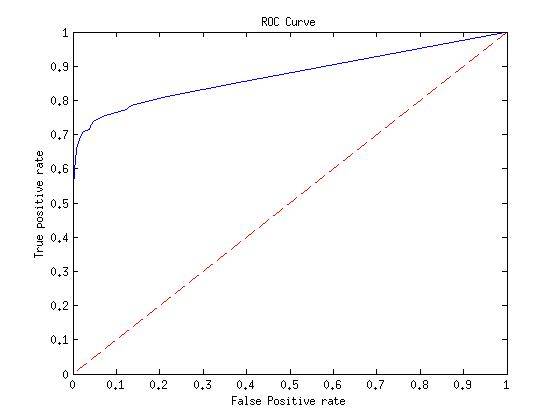
\includegraphics[width=0.6\textwidth]{../Drawings/ROC_SBRISK_SURF2D_Hamming.jpg}
%	\caption{The ROC Curve for SBRISK SURF2D Hamming}
%	\label{fig:sbriskroc}
%\end{figure}


%2. threshold, hammingdistance + KNN
%****************************************************************
%\begin{table}
%\caption{Optimum Threshold}
%\begin{tabular}{|c|c|c|c|c|c|c|c|c|c|c|}
%\hline 
%Detector & Extractor & Matcher & k1 & k2 & k3 & k4 & threshold & distance & thresholdC & distanceC\tabularnewline
%\hline 
%\hline 
%SBRISK & SURF2D & Hamming & 0.6 & 0.4 & 0.4 & 0.6 & 65 & 0.28 & 60 & 0.28\tabularnewline
%\hline 
%\end{tabular}
%\label{tab:sbrisk}
%\end{table}


%\begin{table}
%\caption{Optimum Threshold}
%\begin{tabular}{|c|c|c|c|c|c|c|c|c|}
%\hline 
%\% AUC & Detection(ms) & Extraction(ms) & Matching(ms) & Verification(ms) & Overall(ms) & OP & \% TP & \% FP\tabularnewline
%\hline 
%\hline 
%87.37 & 16.7 & 87.19 & 0.43 & 0.01 & 112.97 &  &  & \tabularnewline
%\hline 
%\end{tabular}
%\label{tab:sbrisk}
%\end{table}


%STATS:
%a. The AUC
%b. average time, extraction, deletion


\subsubsection{S-BRISK}
\label{sec:sbriskResults}
%Find the optimal parameters:
%1. threshold only + KNN
%\begin{table}
%\caption{Optimum Threshold}
%\begin{tabular}{|c|c|c|c|c|c|c|c|c|}
%\hline 
%Detector & Extractor & Matcher & k1 & k2 & k3 & k4 & threshold & thresholdC\tabularnewline
%\hline 
%\hline 
%S-BRISK & S-BRISK & KNN=2 & 0.6 & 0.4 & 0.4 & 0.6 & 46.25 & 30\tabularnewline
%\hline 
%\end{tabular}
%\label{tab:sbrisk}
%\end{table}

%1. Picture of the ROC curve
%STATS:
%a. The AUC
%b. average time, extraction, deletion

%\begin{figure}[h!]
%	\centering
%		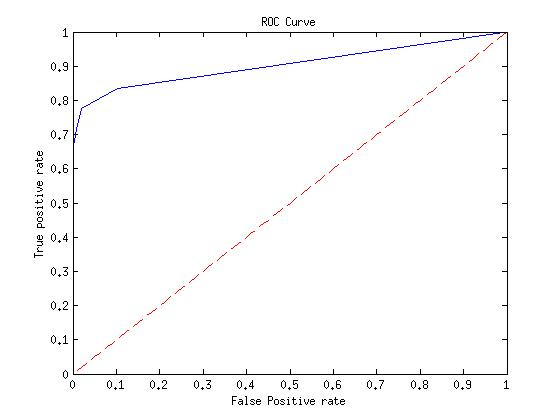
\includegraphics[width=0.6\textwidth]{../Drawings/ROC_SBRISK_SBRISK_KNN.jpg}
%	\caption{The ROC Curve for S-BRISK with KNN}
%	\label{fig:sbriskroc}
%\end{figure}

%\begin{table}
%\caption{Optimum Threshold}
%\begin{tabular}{|c|c|c|c|c|c|c|c|c|}
%\hline 
%\% AUC & Detection(ms) & Extraction(ms) & Matching(ms) & Verification(ms) & Overall(ms) & OP & \% TP & \% FP\tabularnewline
%\hline 
%\hline 
%90.31 & 5.85 & 8.79 & 1.89 & 0.04 & 24.98 &  &  & \tabularnewline
%\hline 
%93.06 & 7.07 & 17.08 & 6.52 & 0.05 & 39.17 &  &  & \tabularnewline
%\hline 
%\end{tabular}
%\label{tab:sbrisk}
%\end{table}


%2. threshold, hammingdistance + KNN
%****************************************************************
%\begin{table}
%\caption{Optimum Threshold}
%\begin{tabular}{|c|c|c|c|c|c|c|c|c|c|c|}
%\hline 
%Detector & Extractor & Matcher & k1 & k2 & k3 & k4 & threshold & distance & thresholdC & distanceC\tabularnewline
%\hline 
%\hline 
%S-BRISK & S-BRISK & Hamming & 0.6 & 0.4 & 0.4 & 0.6 & 78.75 & 110 & 75 & 115\tabularnewline
%\hline 
%\end{tabular}
%\label{tab:sbrisk}
%\end{table}

%\begin{figure}[h!]
%	\centering
%		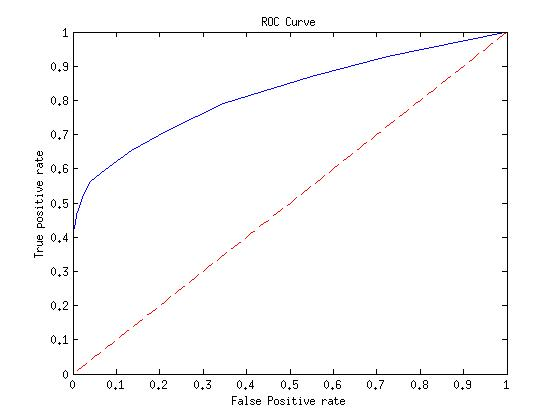
\includegraphics[width=0.6\textwidth]{../Drawings/ROC_SBRISK_SBRISK_Hamming.jpg}
%	\caption{The ROC Curve for S-BRISK using Hamming distance}
%	\label{fig:sbriskrocHamming}
%\end{figure}


%\begin{tabular}{|c|c|c|c|c|c|c|c|c|}
%\hline 
%\% AUC & Detection(ms) & Extraction(ms) & Matching(ms) & Verification(ms) & Overall(ms) & OP & \% TP & \% FP\tabularnewline
%\hline 
%\hline 
%82.24 & 5.15 & 4.62 & 0.33 & 0.01 & 18.63 &  &  & \tabularnewline
%\hline 
%\end{tabular}




%1. Picture of the ROC curve
%STATS:
%a. The AUC
%b. average time, extraction, deletion

\subsubsection{1DSURF}
\label{sec:1dsurfResults}
%1. Picture of the ROC curve
%STATS:
%a. The AUC
%b. average time, extraction, deletion


\subsection{Localisation Performance}
\label{sec:localisationPerformance}







\section{Conclusion}
\label{sec:conclusion}

%\bibliographystyle{witseie}
%\bibliography{bibliography}
% \newpage
%\onecolumn
%\appendix
%\setcounter{table}{0}
%\setcounter{figure}{0}
%\setcounter{subsection}{0}
%\makeatletter \renewcommand{\thefigure}{A.\@arabic\c@figure} \renewcommand{\thetable}{A.\@arabic\c@table} \renewcommand{\thesection}{A.\@arabic\c@section} \makeatother
%\section*{APPENDIX A}
%
%\section{Control Program}
%Add the matlab code to this file...
%\lstinputlisting{codeSnippets.cpp}
 
\end{document}

